\chapter{Космические корабли и станции: современные реалии 50-летней давности}
\label{ch:spacecraft-space-station}

\begin{marginfigure}[2.0cm]
{
	\setlength{\fboxsep}{0pt}%
	\setlength{\fboxrule}{1pt}%
	\fcolorbox{gray}{gray}{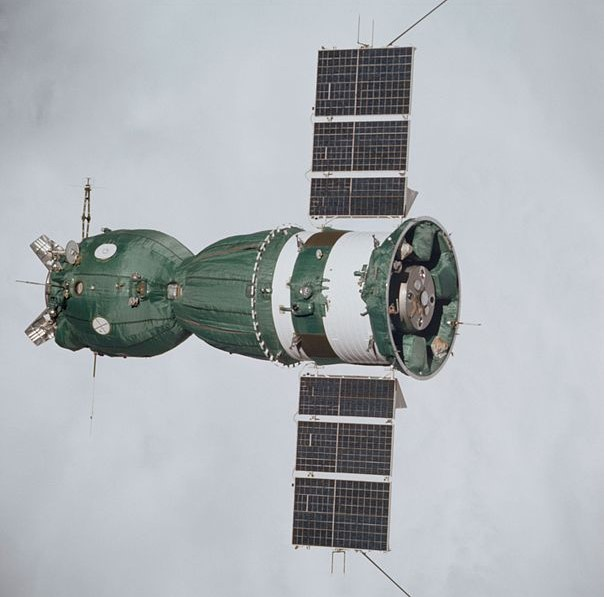
\includegraphics{graphics/chapter/spacecraft_space_station/soyuz-19.jpg}}
}
\caption
[Союз-19, 2021.]
{
В какой стране спроектирован аппарат, изображённый на рисунке?
См. ответ~\ref{answer:spacecraft_USSR} на с.~\pageref{answer:spacecraft_USSR}.
}
\label{question:spacecraft_soyuz19}
\end{marginfigure}

Глава посвящена исследованию космических кораблей и станций на основе Викиданных. 
С помощью SPARQL-скриптов построен список отечественных кораблей и станций, 
нарисованы временные графики запуска кораблей в нашей стране и в мире за период с 1960 по 2021 год. 
Выполнена оценка полноты Викиданных, показавшая, 
что многие объекты имеют неправильное значение свойства 
\wdProperty{31}{частный случай понятия}. В ходе работы было обнаружено, что текущие показатели росийской космонавтики по количеству запусков космических кораблей за последние годы соответствуют показателям в СССР пятьдесят лет назад. 
\marginnote{<<Частный случай понятия>> или <<экземпляр>> 
    (англ. \emph{instance of})~--- это конкретный объект класса, категории, 
    это одно из основных свойств (отношений), используемых в Викиданных и позволяющих классифицировать объекты, 
    соотносить их разным <<классам>>, <<категориям>>.%
}

\section{Список космических кораблей и станций}

Построим запрос~\ref{lst:spaceships} для вывода списка всех космических кораблей и станций. 
Нам потребуются объекты \wdqName{космическая станция}{25956}, 
\wdqName{космический корабль}{40218} и отношение \wdProperty{31}{экземпляр}. 

\index{SPARQL!VALUES!Список кораблей и станций}
\index{SPARQL!SERVICE!Список кораблей и станций}
\begin{lstlisting}[ language=SPARQL, numbers=none, caption={{\href{https://w.wiki/4d4f}{Список кораблей и станций}}\protect\footnotemark}, label=lst:spaceships, ]
# List of spacecraft (Q40218) and space station (Q25956)
SELECT  ?s ?sLabel ?typeLabel
WHERE
{
  VALUES ?type {wd:Q40218 wd:Q25956}
  ?s wdt:P31 ?type.  # Selecting the type of object
  SERVICE wikibase:label {bd:serviceParam wikibase:language"ru,en"}
}
\end{lstlisting}
\footnotetext{Найдено \num{145} объектов в 2021 году. SPARQL-запрос: \url{https://w.wiki/4d4f}}


\section{Глубина проработки объектов}

По состоянию на 2021 год на Викиданных 
наиболее полным и проработанным является космический корабль 
\wdqName{Аполлон-8}{184201}, 
имеющий 30 свойств\autocite{spacecraftProWD}. 
При этом всего всего по одному свойству имеют такие корабли, как: 
\wdqName{Europa Astrobiology Lander}{10491365}, 
\wdqName{Project Orbiter}{6514453}, 
\wdqName{LRK}{5961734}, 
\wdqName{EarthForce One}{5327028}\sidenote[][]{%
%
Отметим непростую судьбу объекта \wdqName{EarthForce One}{5327028}. 
Этот объект был создан в Викиданных ботом автоматически в 2013 году, 
поскольку существовала статья в Английской Википедии. 
Как написано на странице ``\href{https://en.wikipedia.org/wiki/EarthForce_One}{EarthForce One}'' 
в Английской Википедии, статья была удалена из-за отсутствия надёжных источников, 
доказывающих значимость объекта. 
А в Викиданных объект остался как неприкаянный. 
Подумайте над запросом, который вывел бы список аналогичных объектов Викиданных, 
не соответствующих ни одной статье Википедии.%
%
}, 
\wdqName{Союз ГВК}{60767924}, 
\wdqName{CubeSat for Solar Particles}{22907583}\autocite{spacecraftProWD}. 
Для поиска этой информации был использован запрос, построенный с помощью сервиса ProWD\autocite{spacecraftProWD}. 
Этот же сервис показал, что заполнение космических объектов неравномерное, 
большая часть заполнены менее, чем на 30\%\autocite{spacecraftProWD}. 

\section{Список отечественных кораблей и станций}

\begin{marginfigure}
{
	\setlength{\fboxsep}{0pt}%
	\setlength{\fboxrule}{1pt}%
	\fcolorbox{gray}{gray}{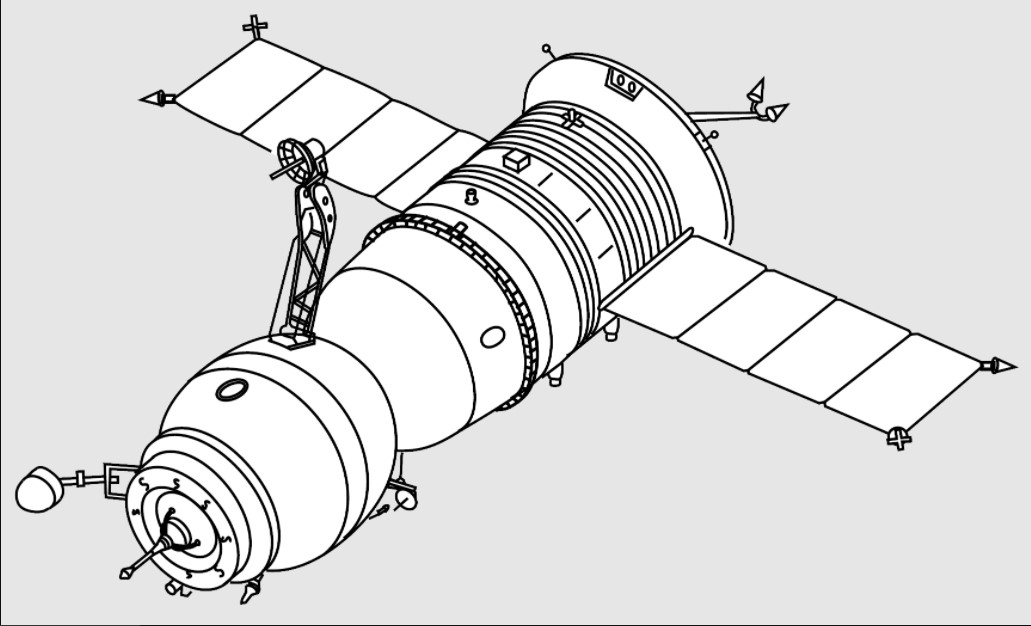
\includegraphics{graphics/chapter/spacecraft_space_station/soyuz-t.jpg}}
}
\caption
[Союз-T, 2021.]
{
В какой стране спроектирован аппарат, изображённый на рисунке?
См. ответ~\ref{answer:spacecraft_USSR} на с.~\pageref{answer:spacecraft_USSR}.
}
\label{question:spacecraft_soyuzT}
\end{marginfigure}

Найдём корабли и станции, сконструированные в СССР или России, 
с помощью запроса~\ref{lst:spaceshipsUSSR}.

\index{SPARQL!SERVICE!Список отечественных кораблей}
\begin{lstlisting}[ language=SPARQL, 
                    numbers=none, 
                    caption={{\href{https://w.wiki/4d9c}{Список отечественных кораблей}}\protect\footnotemark}, 
                    label=lst:spaceshipsUSSR
                  ]
# List of Russian and USSR spacecrafts and stations
SELECT  ?spacecraft  ?spacecraftLabel 
WHERE
{
  {?spacecraft wdt:P31 wd:Q40218.} UNION #spacecraft
  {?spacecraft wdt:P31 wd:Q25956.} # and space station
  
  # Soviet Union and Russia
  VALUES ?ruCountries {wd:Q15180 wd:Q159}
  ?spacecraft wdt:P17 ?ruCountries. # related to Russian countries
  
  SERVICE wikibase:label {bd:serviceParam wikibase:language "ru,en"}
}
\end{lstlisting}
\footnotetext{Найдено три отечественных корабля и станции 
в 2017 году и \num{25}~--- в 2021 году. SPARQL-запрос: \href{https://w.wiki/4BbY}{https://w.wiki/4d9c}}


\section{Анализ полноты Викиданных}

Проанализируем степень заполнения Викиданных в области отечественных космических кораблей и станций. 
Если по запросу~\ref{lst:spaceships} обо всех кораблях и станциях было получено 145 результатов, 
то по запросу~\ref{lst:spaceshipsUSSR} об отечественных объектах~--- всего 25. Информации о советских и российских объектов в 2021 стало в несколько раз больше по сравнению с 2017 годом, когда по запросу~\ref{lst:spaceshipsUSSR} выдавалось всего 3 объекта. 

На сайте Буран.Ру в разделе кораблей СССР и России по состоянию на 2021 год содержится информация о 36 кораблях\autocite{spacecraftBuran}. В советской энциклопедии <<Космонавтика>> от 1985 года упоминаются запуски 1992 советских космических объектов 24 различных типов в период с 1957 по 1984 год\autocite[~498]{spacecraftCosmonavtika}. 
В американском справочнике по космонавтике и астрономии книге приведены всего 10 советских и российских запусков космических станций\autocite[~296]{spacecraftSAA}, 126 запусков шатла у НАСА в период с 1981 по 2008 год \autocite[~288]{spacecraftSAA}, и 31 международный запуск\autocite[~290---291]{spacecraftSAA}. 

\section{Временные графики освоения космоса в~нашей стране и мире}

\begin{marginfigure}
{
	\setlength{\fboxsep}{0pt}%
	\setlength{\fboxrule}{1pt}%
	\fcolorbox{gray}{gray}{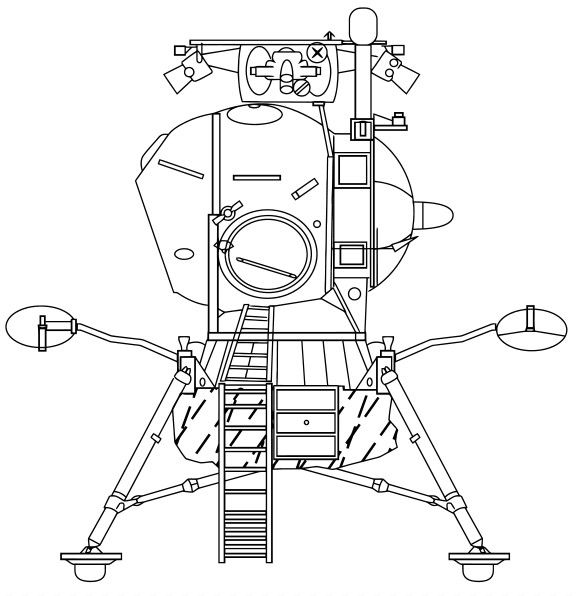
\includegraphics{graphics/chapter/spacecraft_space_station/lunar_landler.jpg}}
}
\caption
[Лунный корабль, 2021.]
{
В какой стране спроектирован аппарат, изображённый на рисунке?
См. ответ~\ref{answer:spacecraft_USSR} на с.~\pageref{answer:spacecraft_USSR}.
}
\label{question:spacecraft_lunar}
\end{marginfigure}

Временной (с 1960-х годов) 
график запуска космических аппаратов в нашей стране (рис.~\ref{fig:launchesRussia5years}) 
построен с помощью запроса~\ref{lst:launchesRussia5years}.%

Ранее в запросах для получения каких-либо списков мы использовали свойство \wdProperty{31}{экземпляр}. 
В запросе~\ref{lst:launchesRussia5years} мы обошлись без этого свойства за счёт использования отношения 
\wdProperty{619}{<<дата запуска космического корабля>>} в строке 10 
для обхода и подсчёта таких объектов, которые были запущены в космос.  

Логический оператор \lstinline|UNION| в строках 5--8 
позволяет объединить советские и российские запуски космолётов. 

Если бы в запросе вместо переменной \lstinline|?lapse| оставалась~--- \lstinline|?year| (строки 3 и 12), 
то мы получили бы на рис.~\ref{fig:launchesRussia5years} 
число запусков за каждый год. 
Благодаря функции округления \lstinline|FLOOR()|
и группировке%
\sidenote[][]{
%
В строке 15 запроса~\ref{lst:launchesRussia5years} 
запущенные в космос объекты группируются командой: 
\mbox{\lstinline|GROUP BY ?lapse|.}\newline
То, что группировка идёт именно по пятилеткам, а не, например, шестилеткам, 
определяется в строке 12, где переменная \lstinline|?year| делится на 5, округляется и умножается на 5.%
%
}, 
объекты \lstinline|?item|, имеющие запуски, группируются за пятилетний период, 
и в переменную \lstinline|?quantity| записывается число этих объектов, 
подсчитанное с помощью функции \lstinline|COUNT()|.

Для представления результатов в виде столбчатой диаграммы используется стиль отображения BarChart.

\label{question:spacecraft_1}
\marginnote[3cm]{
%%%%%%%%%%%%%%%% Упражнение 1 %%%%%%%%%%%%%%%% 
Сколько кораблей было запущено в~СССР в~1960-е, 1970-е и 1980-е годы?

См. ответ~\ref{answer:launches_USSR} на с.~\pageref{answer:launches_USSR}.
}

\index{SPARQL!STR!Запуски космических кораблей в СССР и России}
\index{SPARQL!BIND!Запуски космических кораблей в СССР и России}
\index{SPARQL!YEAR!Запуски космических кораблей в СССР и России}
\index{SPARQL!FLOOR!Запуски космических кораблей в СССР и России}
\index{SPARQL!UNION!Запуски космических кораблей в СССР и России}
\index{SPARQL!COUNT!Запуски космических кораблей в СССР и России}
\index{SPARQL!GROUP BY!Запуски космических кораблей в СССР и России}
\index{SPARQL!ORDER BY!Запуски космических кораблей в СССР и России}
\begin{lstlisting}[ language=SPARQL, 
                    caption={{\href{https://w.wiki/4QGX}{Запуски космических кораблей в СССР и России}}\protect\footnotemark}, 
                    label=lst:launchesRussia5years,
                    texcl
                  ]
# The number of spacecraft launches in Russia every 5 years
#defaultView:BarChart
SELECT (STR(?lapse) AS ?lapse_str) (COUNT(?item) AS ?quantity)
WHERE {                                  # spacecraft belongs to
        {?item wdt:P17 wd:Q15180}               # country = USSR
  UNION {?item wdt:P17 wd:Q159}               # country = Russia
  UNION {?item wdt:P495 wd:Q159}    # country of origin = Russia
  UNION {?item wdt:P495 wd:Q15180}.  # country of origin =  USSR
  
  ?item wdt:P619 ?launch. # date of spacecraft launch
  BIND( YEAR(?launch) AS ?year) 
  BIND(FLOOR(?year/5)*5 AS ?lapse) # count for each 5 years
SERVICE wikibase:label {bd:serviceParam wikibase:language "ru,en"}
} 
GROUP BY ?lapse
ORDER BY ?lapse # Order 1970, 1975, 1980, ...
\end{lstlisting}
\footnotetext{Найдено \num{14} пятилеток. SPARQL-запрос: \href{https://w.wiki/4eGg}{https://w.wiki/4eGg}}

\index{График!BarChart!Количетво запусков космических кораблей в СССР и России каждые 5 лет}
\begin{figure*}[h!]
  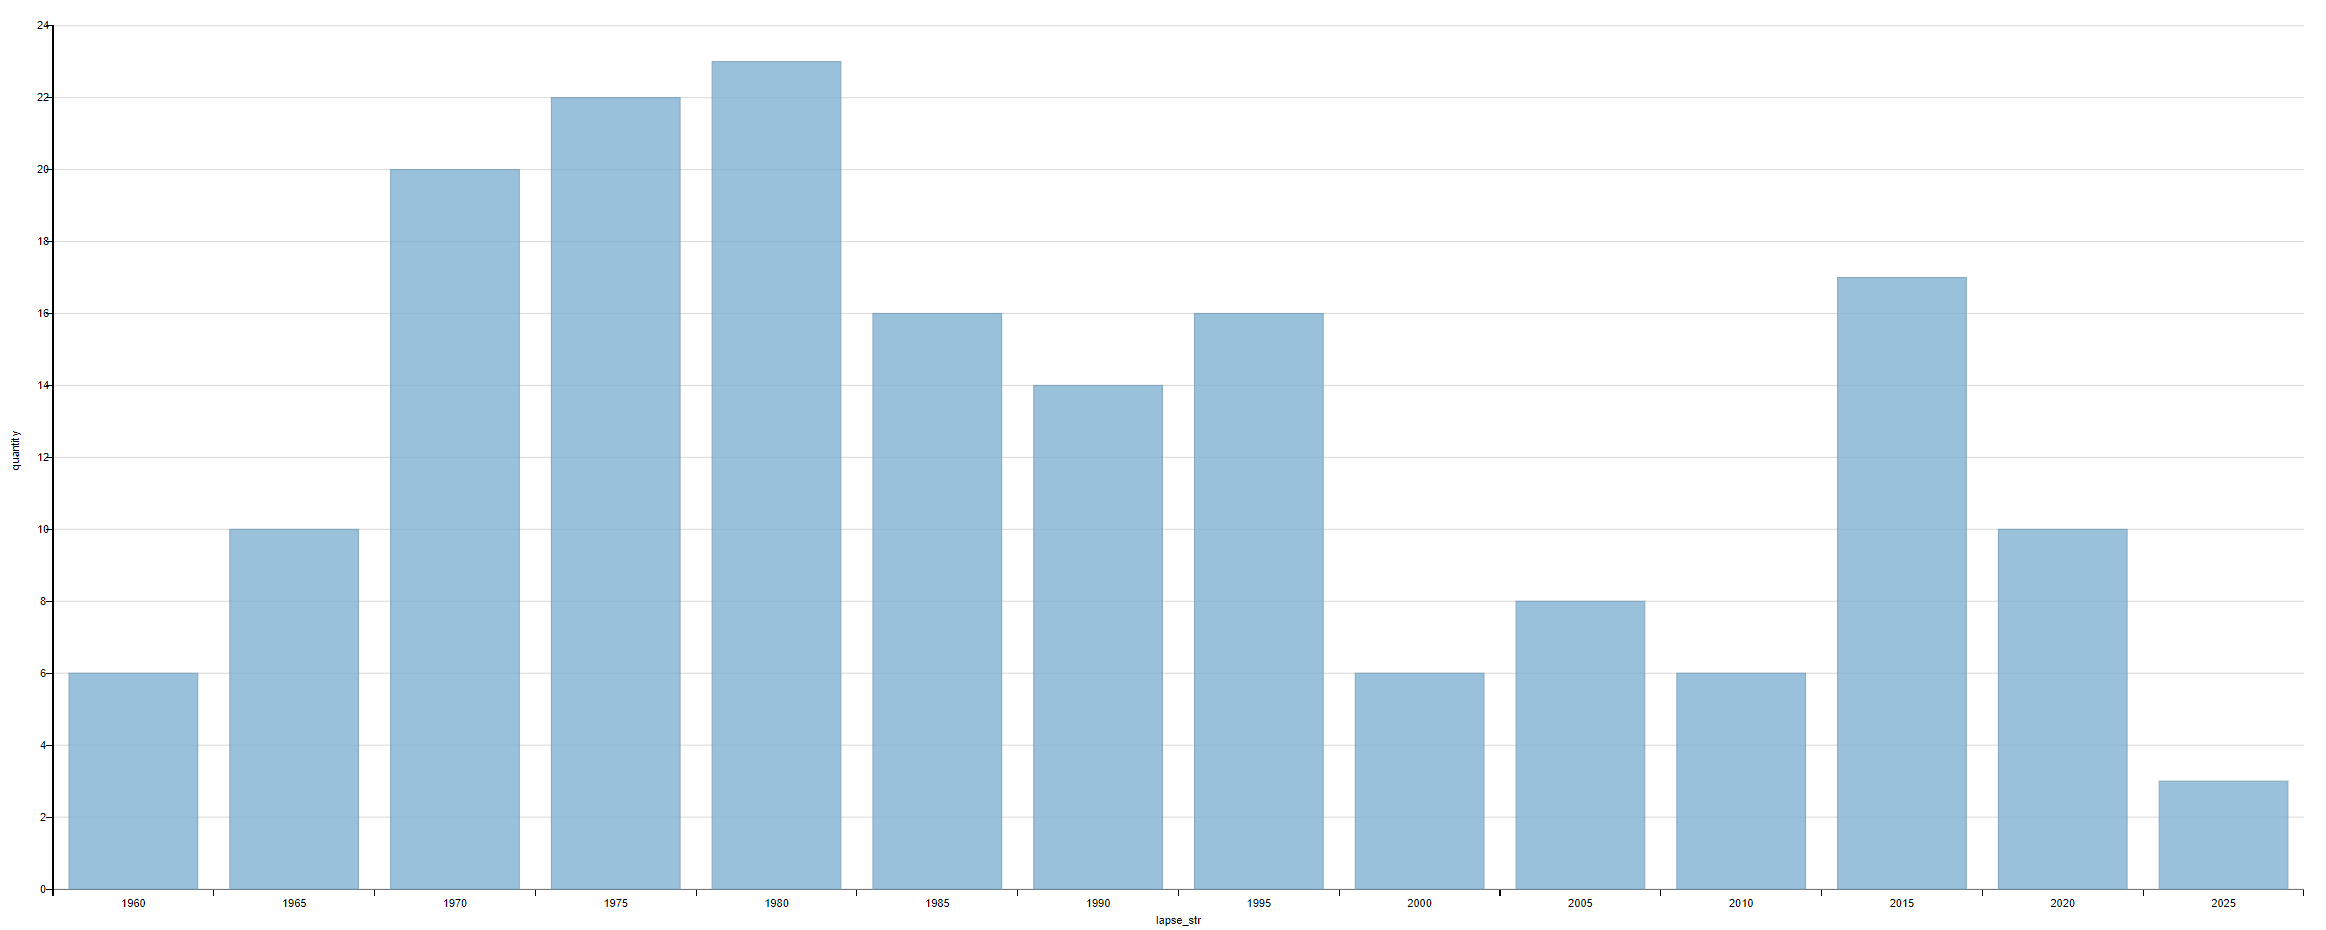
\includegraphics[width=\linewidth]{graphics/chapter/spacecraft_space_station/Visualization of the number of spacecraft launches in USSR and Russia per 5 years 2022.png}
  \caption[График запусков космических кораблей в СССР и России (по пятилеткам )]{Визуализация количества запусков космических кораблей в СССР и России каждые 5 лет, построено с помощью скрипта~\protect\ref{lst:launchesRussia5years} в 2022 году.}%
  \label{fig:launchesRussia5years}%
\end{figure*}

Горизонтальной ос\'{и} на рис.~\ref{fig:launchesRussia5years} отвечает переменая \mbox{\lstinline|?lapse_str|.} 
Если не преобразовывать число \lstinline|?lapse| 
в текстовую переменную \mbox{\lstinline|?lapse_str|}%
\sidenote[][]{
%
Преобразование числа в текст  
в третьей строке запроса~\ref{lst:launchesRussia5years}:\newline
\lstinline|(STR(?lapse) AS ?lapse_str)|.%
%
}, то ось~X имеет диапазон от 0 до 2200, 
вместо требуемого диапазона от 1960 до 2025 года, 
а результаты обозначаются точками с координатами (пятилетка, число запусков), 
и график становится нечитаемым. 

Из рис.~\ref{fig:launchesRussia5years} видно, 
что самый активный период развития отечественной космонавтики был в 1970--1995 годах.

Запрос~\ref{lst:launchesWorld} строит график~\ref{fig:launchesWorld} 
запусков космических кораблей в~мире по годам и странам.

\index{SPARQL!COUNT!Запуски космических кораблей в мире}
\index{SPARQL!YEAR!Запуски космических кораблей в мире}
\index{SPARQL!BIND!Запуски космических кораблей в мире}
\index{SPARQL!SERVICE!Запуски космических кораблей в мире}
\index{SPARQL!GROUP BY!Запуски космических кораблей в мире}
\begin{lstlisting}[ language=SPARQL, 
                    numbers=none, 
                    caption={{\href{https://w.wiki/4bEu}{Запуски космических кораблей в мире}}\protect\footnotemark}, 
                    label=lst:launchesWorld
                  ]
# Diagram of spacecraft launches by year and country
#defaultView:BarChart
SELECT ?year (COUNT(?obj) AS ?count) ?country ?countryLabel
WHERE {
  ?obj wdt:P17 ?country. # spacecraft belongs to country 
  ?obj wdt:P619 ?launch. # date of spacecraft launch
  BIND(str(YEAR(?launch)) AS ?year)
  
  SERVICE wikibase:label {bd:serviceParam wikibase:language "ru".}
}
GROUP BY ?year ?country ?countryLabel
\end{lstlisting}
%%%%%%%%%%%%%%%% Упражнение 2 %%%%%%%%%%%%%%%% 
\label{question:spacecraft_2}
\marginnote[-4cm]{%
В какое наибольшее и наименьшее количество запусков космических кораблей за десятилетие совершило человечество в период с 1970 по 2010 годы?

См. ответ~\ref{answer:launches_world} на с.~\pageref{answer:launches_world}.
}
\footnotetext{Найдено \num{328} результатов в 2021 году. Ссылка на SPARQL-запрос: \href{https://w.wiki/4bEu}{https://w.wiki/4bEu}}

\index{График!BarChart!Визуализация количества запусков космических кораблей по годам и странам}
\begin{figure*}[h!]
  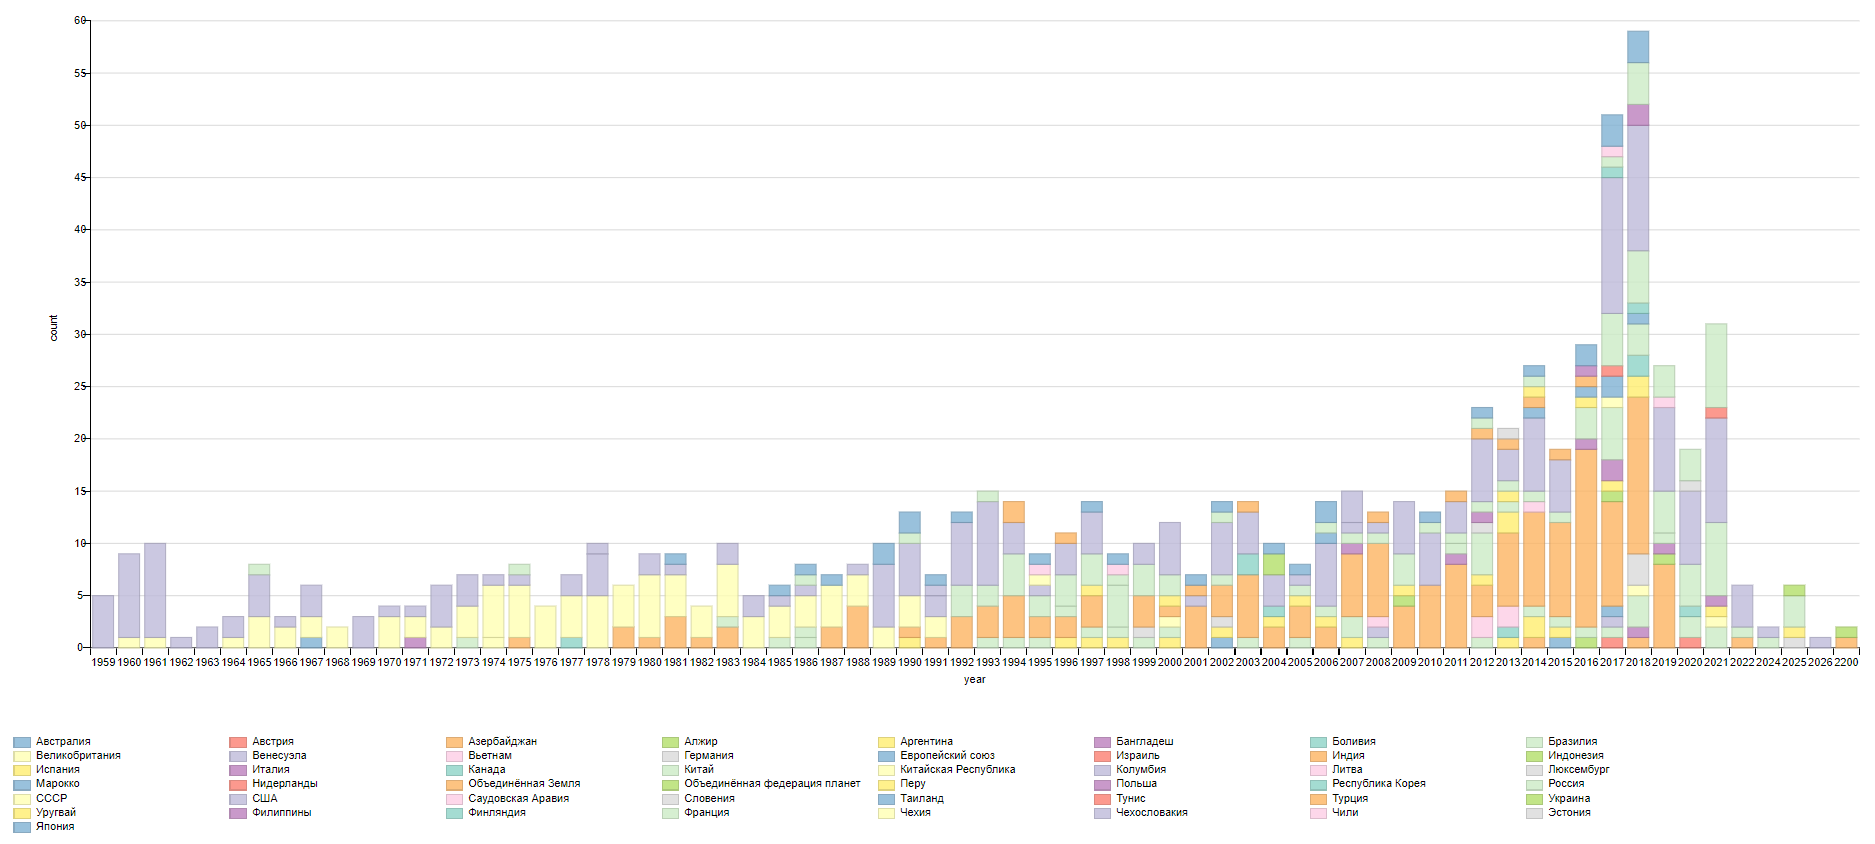
\includegraphics[width=\linewidth]{graphics/chapter/spacecraft_space_station/Visualization of the number of spacecraft launches by year and country 2021.png}
  \caption[График запусков космических кораблей во всём мире по годам и странам]{Визуализация количества запусков космических кораблей по годам и странам, построено с помощью скрипта~\protect\ref{lst:launchesWorld} в 2021 году.}
  \label{fig:launchesWorld}%
\end{figure*}

Из рис.~\ref{fig:launchesWorld} видно, что больше всего космических аппаратов 
запускали Индия и США 
(только у них зафиксировано более 10 ежегодных запусков) в 2017--2018 годах. 
Пик запусков в мире был в 2018 году (59 запусков). 

По Викиданным российская космонавтика занимает средние позиции по количеству запусков, 
её численные показатели за 2016--2019 годы схожи с показателями СССР в 1970-е и 1980-е годы 
и составляют 3--5 запусков в год.

\section{Космонавты в международных полётах}

Запрос~\ref{lst:internationalFlights} строит граф~\ref{fig:internationalFlights} c вершинами типа <<ракеты>> и <<космонавты>> с раскраской по странам.

\index{SPARQL!DISTINCT!Космонавты в международных полётах}
\index{SPARQL!SERVICE!Космонавты в международных полётах}
\index{SPARQL!BIND!Космонавты в международных полётах}
\index{SPARQL!VALUES!Космонавты в международных полётах}
\begin{lstlisting}[ language=SPARQL, caption={{\href{https://clck.ru/agMjd}{Космонавты в международных полётах}}\protect\footnotemark}, 
                    label=lst:internationalFlights
                  ]
# Graph of astronauts as crew of flights of different countries
#defaultView:Graph
SELECT DISTINCT ?item ?itemLabel ?rgb ?link ?naut_seed
WHERE
{ 
  VALUES ?toggle { true false }
  # Let's select a subset of astronauts
  {
    SELECT DISTINCT ?naut WHERE
    { 
      VALUES ?naut_seed {wd:Q313815}.  # Sergei Krikalev
      ?s wdt:P1029 ?naut_seed, ?naut;  
    }       # ?naut_seed & ?naut are member of a same crew
  }
  ?s  wdt:P31/wdt:P279* wd:Q40218; # spacecraft and subclasses
      wdt:P31/wdt:P279* wd:Q752783;# human spaceflight and subclasses
          wdt:P1029 ?naut;         # has member of the crew ?naut    
  SERVICE wikibase:label {bd:serviceParam wikibase:language "en"}
  BIND(IF(?toggle,?s,?naut) AS ?item).
  BIND(IF(?toggle,?sLabel,?nautLabel) AS ?itemLabel).
  BIND(IF(?toggle,"FFFFFF","7FFF00") AS ?rgb_source).
  BIND(IF(?toggle,"",?s) AS ?link).
  ?naut wdt:P27 ?country. # astronaut is citizen of country 
  # ?toggle = true then spacecraft node
  # ?toggle = false then astronaut node
  BIND(             # Soviet & Russian astronauts have red nodes
    IF(!?toggle && (?country=wd:Q15180||?country=wd:Q159),"FF0000",
    IF(!?toggle && ?country=wd:Q30,"FF00FF",  # USA - fuchsia
    IF(!?toggle && ?country=wd:Q183,"C0C0C0", # Germany - silver
    IF(!?toggle && ?country=wd:Q142,"008080", # France - teal
    IF(!?toggle && ?country=wd:Q40,"800000", # Austria - maroon
    IF(!?toggle && ?country=wd:Q38,"00FFFF", # Italy - aqua
    ?rgb_source))))))
    AS ?rgb).
}
\end{lstlisting}
\footnotetext{Найдено \num{68} результатов в 2022 году. Ссылка на SPARQL-запрос: \href{https://clck.ru/agMjd}{https://clck.ru/agMjd}}

Для работы скрипта необходимо указать начальную точку~-- космонавта, который принимал участие в международных космических полётах. Начальная точка задаётся в строке 11 скрипта и записывается в переменную \lstinline|?naut_seed|. Далее, в строке 12, выполняется поиск астронавтов, летавших совместно с тем, кого мы указали ранее. В строках 15--17 подгружаются данные о космических аппаратах, полётах и астонавтах. Булевая переменная \lstinline|?toggle| имеет значение \lstinline|?true|, если найденный объект является космическим аппаратом или  \lstinline|?false|, если найденный объект является космонавтом. В переменную \lstinline|?item| в девятнадцатой строке записывается айди объекта на Викиданных. В строке 20 в переменную \lstinline|?itemLabel| записывается название объекта, в строке 21 в переменную \lstinline|?rgb_source| записываются данные для раскраски кораблей, в строке 22 в переменную \lstinline|?link| записывается айди корабля, благодаря которому мы перешли на данного космонавта. В строке 23 подгружаются данные о гражданстве  космонавта, а в строках 26--34 космонавтам присваивается цвет в зависимости от их гражданства. 

\index{График!Graph!Космонавты в международных полётах}
\begin{figure*}[h]
  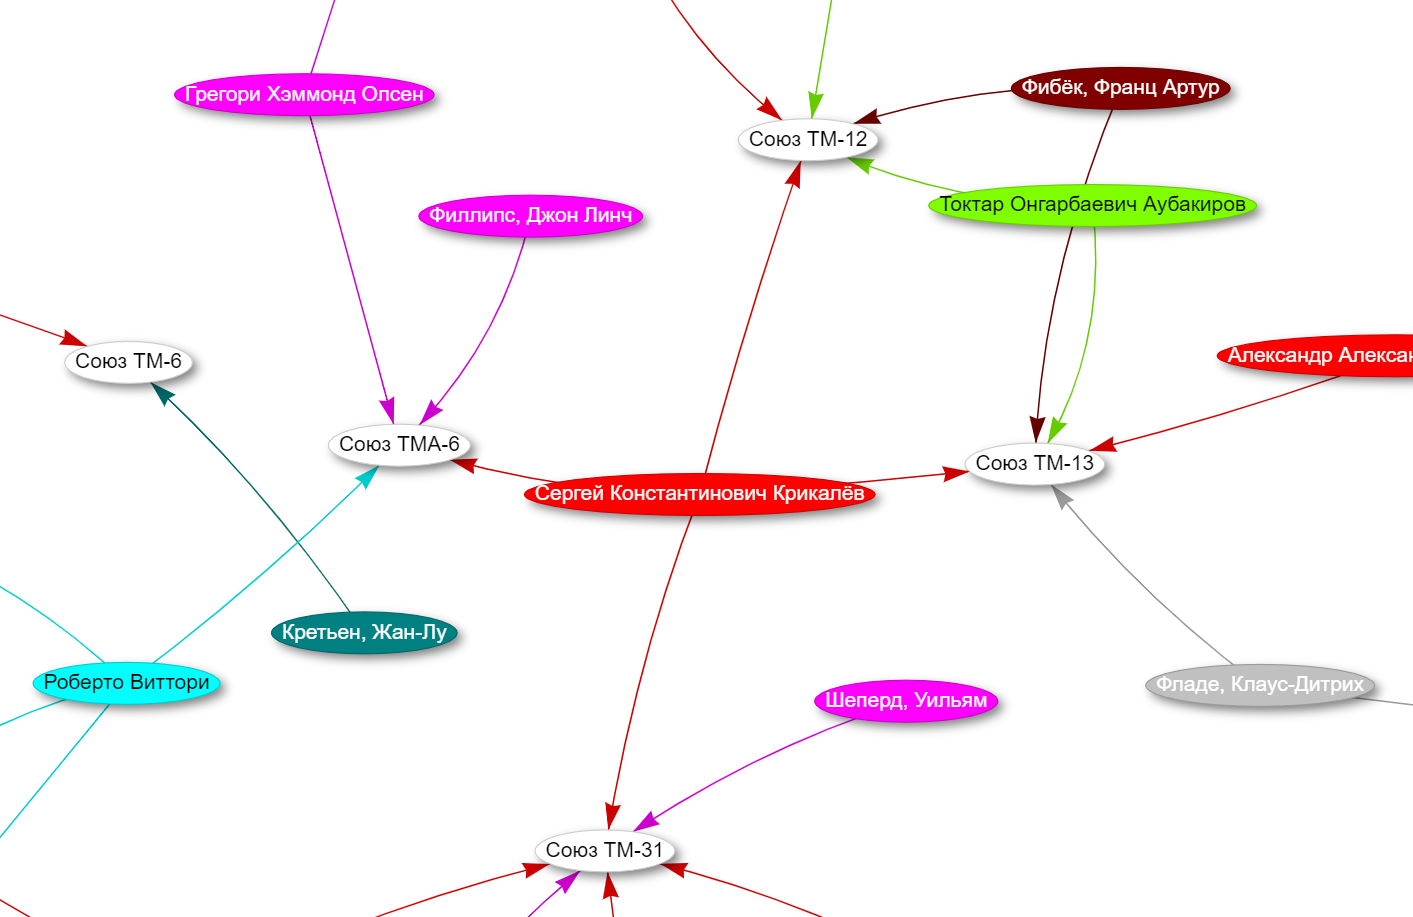
\includegraphics[width=\linewidth]{graphics/chapter/spacecraft_space_station/Cosmonauts in international flights RU.png}
  \caption[Граф c вершинами типа <<ракеты>> и <<космонавты>> с раскраской по странам]{Граф c вершинами типа <<ракеты>> и <<космонавты>> с раскраской по странам. Красный цвет соответствует СССР и России, розовый~--- США, серый~--- Германии, бирюзовый~--- Франции, бордовый~--- Австралии, а голубой~--- Италии. Граф построен с помощью скрипта~\protect\ref{lst:internationalFlights} в 2022 году.}
  \label{fig:internationalFlights}%
\end{figure*}

\section{Упражнения}
\begin{enumerate}
  \item Постройте список кораблей, которые отправились или отправятся на \wdqName{Марс}{111}.
  \item Подсчитайте долю кораблей (нарисуйте график по десятилетиям), 
        отправленным на \wdqName{Марс}{111}, 
        по отношению к числу кораблей, отправленных на \wdqName{Луну}{405}.
  \item Подсчитайте количество \wdqName{успешных}{7632586} космических запусков 
      относительно \wdqName{неудачных}{1121708}.%
\marginnote[-32pt]{%
Например, у объекта \wdqName{<<космическая программа Луна>>}{192372} 
в свойстве \wdProperty{793}{<<ключевое событие>>} 
указано число успешных и неудачных запусков.%
}%
\end{enumerate}
